\documentclass{article}

\usepackage{titlesec}
\newcommand{\sectionbreak}{\clearpage}

\usepackage{fancyhdr}
\pagestyle{fancy}
\lhead{Emanuel Casiano-Diaz}
\rhead{CSYS300: PoCS - Homework 02 - 09/15/2018}
\renewcommand{\headrulewidth}{0.4pt}
\renewcommand{\footrulewidth}{0.4pt}

\usepackage{amsmath}
\usepackage{amssymb}
\usepackage{bm}
\usepackage{pdfpages}

\usepackage{enumerate}% http://ctan.org/pkg/enumerate

\usepackage{hyperref}
\hypersetup{
    colorlinks=true,
    linkcolor=blue,
    filecolor=magenta,      
    urlcolor=cyan,
}


\begin{document}

Code used throughout the assignment can be found in the following git repository: \url{https://github.com/ecasiano/PrinciplesOfComplexSystems} \\

\section{Exercise 1}

\begin{figure}[h!]
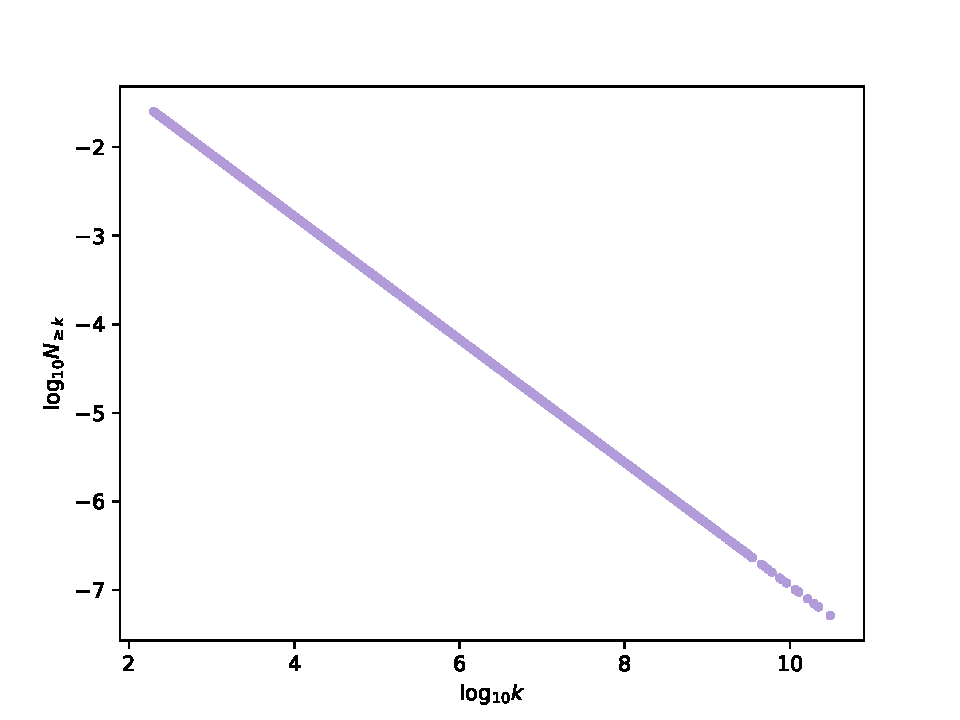
\includegraphics[width=\linewidth]{Q01/wordFrequencyCCDFLog.pdf}
\caption{Logarithm of the complementary cumulative distribution of $N_k$ with respect to the frequencies, $k$. }
\label{fig:ccdf}
\end{figure}

\section{Exercise 2}

The following values correspond to the $N_k$ values in the previous figure: \\
\\
CCDF exponent: $\gamma-1 = 0.6951$ with $r^2 = 0.99455$\\
Mean$^*$: $\mu_{N_k} = 3.36372e+06$\\
Standard Deviation$^*$: $\sigma_{N_k} =1.26384e+08$\\
$95\%$ Confidence Interval$^{**}$ : $[2.84624e+06,3.88120e+06]$\\
\\
$*$ Mean and Standard Deviation correspond to the full distribution, not only on the range shown.\\
\\
$**$ Obtained via $\mu_{N_k} \pm \frac{2\sigma_{N_k}}{\sqrt{size(k)}}$ 

\section{Exercise 3} 

\begin{figure}[h!]
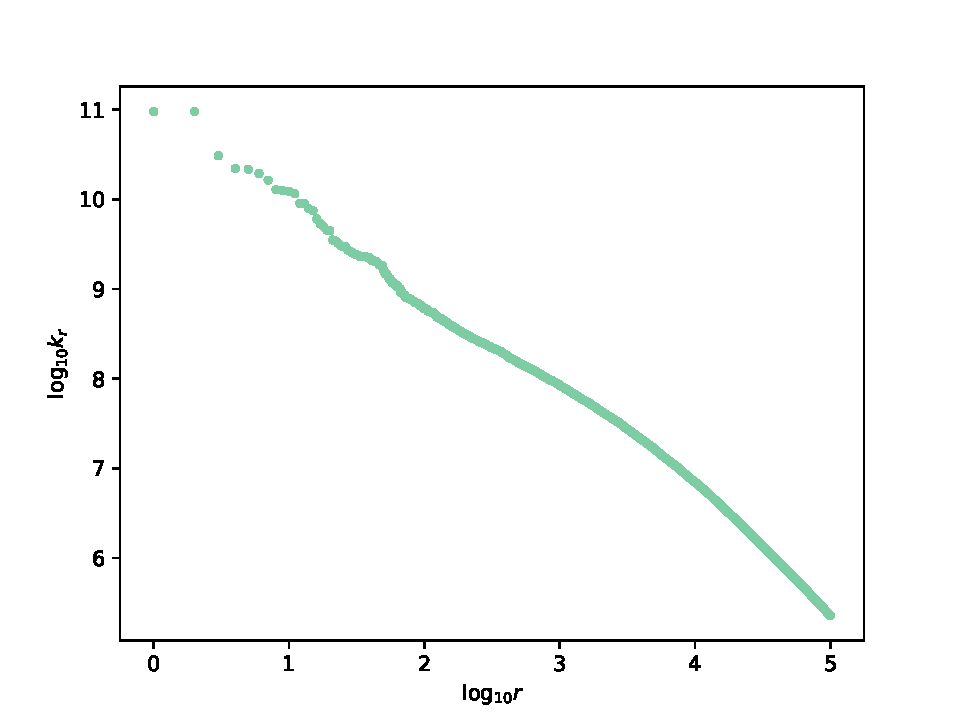
\includegraphics[width=\linewidth]{Q03/zipfRanksLog.pdf}
\caption{Logarithm of the word frequencies, $k_r$ with respect to the logarithm of their rank, $r$. }
\label{fig:zipf}
\end{figure}

\section{Exercise 4}

The following values correspond to the $k_r$ values in the previous figure: \\
\\
Zipf's exponent: $\alpha = 1.41427563$ with $r^2 = 0.99961232$\\
Mean$^*$: $\mu_{k_r} = 7.54253e+04$\\
Standard Deviation$^*$: $\sigma_{k_r} = 4.01540e+07$\\
$95\%$ Confidence Interval$^{**}$ : $[5.36394e+04,9.72111e+04]$\\
\\
$*$ Mean and Standard Deviation correspond to the full distribution, not only on the range shown.\\
\\
$**$ Obtained via $\mu_{k_r} \pm \frac{2\sigma_{k_r}}{\sqrt{size(k)}}$ 

\section{Exercise 5} 

The rank distribution exponent and the size distribution exponents are related via: \\
\[ \alpha = \frac{1}{\gamma-1} \]
\\
In the previous questions, it was seen that the Zipf exponent was $\alpha \approx 1.41427563$ and $\gamma-1 \approx 0.6951$. Thus the right hand side becomes:
\[ \frac{1}{\gamma-1} \approx 1.43864192\]
and
\[ \alpha \approx 1.41427563 \]
\\
The relative error between the two expressions is then:
\[ | \frac{1.43864192 - 1.41427563}{1.43864192}| X 100 \approx 1.69 \%\]


\end{document}